

\documentclass{beamer}
\usetheme{default}
\usecolortheme{dove}
\usepackage{graphicx}
\usepackage{xcolor}
\usepackage{multicol}
\newcommand\independent{\protect\mathpalette{\protect\independenT}{\perp}}
\newcommand\indep{\protect\mathpalette{\protect\independenT}{\perp}}
\def\independenT#1#2{\mathrel{\rlap{$#1#2$}\mkern2mu{#1#2}}}
\definecolor{dblue}{RGB}{0,0,139}
\usepackage{tikz}
\usetikzlibrary{arrows,shapes.arrows,positioning,shapes,shapes.misc}
\usetikzlibrary{decorations.pathreplacing}
\usepackage{booktabs}
\renewcommand{\arraystretch}{1.2}
\newcommand{\Cov}{\text{Cov}}
\newcommand{\Cor}{\text{Cor}}
\newcommand{\V}{\mathbb{V}}
\renewcommand{\P}{\mathbb{P}}
\newcommand{\E}{\mathbb{E}}
\newcommand{\doop}{\text{do}}
\usepackage{hanging}% http://ctan.org/pkg/hanging
\setbeamertemplate{footnote}{%
  \hangpara{2em}{1}%
  \makebox[2em][l]{\insertfootnotemark}\footnotesize\insertfootnotetext\par%
}
\newcommand{\myfootnote}{\let\thefootnote\relax\footnote}
\newcommand{\blue}[1]{\textcolor{blue}{#1}}
\newcommand{\gray}[1]{\textcolor{gray}{#1}}
\newcommand{\green}[1]{\textcolor{olive}{#1}}
\newcommand{\purple}[1]{\textcolor{purple}{#1}}
\newcommand{\bred}[1]{\textbf{\textcolor{red}{#1}}}
\newcommand{\bblue}[1]{\textbf{\textcolor{blue}{#1}}}
\newcommand{\bgreen}[1]{\textbf{\textcolor{olive}{#1}}}
\newcommand{\bpurple}[1]{\textbf{\textcolor{purple}{#1}}}
\newcommand\black[1]{\color{black}#1}
\newcommand\white[1]{\color{white}#1}
\usepackage{array}
\newcolumntype{L}[1]{>{\raggedright\let\newline\\\arraybackslash\hspace{0pt}}m{#1}}
\usepackage[round]{natbib}
\bibliographystyle{humannat-mod}
\setbeamertemplate{footnote}{%
  \footnotesize\insertfootnotetext\par%
}
\setbeamertemplate{enumerate items}[default]
\usepackage[append]{beamersubframe}
\title{Consistency}
\author{Ian Lundberg}
\institute[Princeton University] % (optional, but mostly needed)
{
  Department of Sociology and Office of Population Research\\
  Princeton University
}
\date{\today}

\begin{document}

\begin{frame}
\centering
\begin{tikzpicture}[x = .5\textwidth, y = .5\textheight]
\node at (-1,-1) {};
\node at (1,1) {};
\node[font={\large\bf},blue,align=center] at (0,.8) {Government assistance protects low-income families\\from eviction and rent nonpayment};
\node (ian) at (-.65,0.5) {Ian Lundberg};
\node (sarah) at (0,0.5) {Sarah L. Gold};
\node (louis) at (.65,0.5) {Louis Donnelly};
\node (brooke) at (-.4,0.1) {Jeanne Brooks-Gunn};
\node (sara) at (.4,0.1) {Sara S. McLanahan};
\node[anchor = north, font = \tiny, align = center, outer sep = -4pt] at (ian.south) {Department of Sociology\\Office of Population Research\\Princeton University};
\node[anchor = north, font = \tiny, align = center, outer sep = -4pt] at (sarah.south) {Office of Population Research\\Princeton University};
\node[anchor = north, font = \tiny, align = center, outer sep = -4pt] at (louis.south) {Office of Population Research\\Center for Research on Child Wellbeing\\Princeton University};
\node[anchor = north, font = \tiny, align = center, outer sep = -4pt] at (brooke.south) {Teachers College\\College of Physicians and Surgeons\\Columbia University};
\node[anchor = north, font = \tiny, align = center, outer sep = -4pt] at (sara.south) {Department of Sociology\\Office of Population Research\\Center for Research on Child Wellbeing\\Princeton University};
\node[align=center] at (0,-.35) {Annual Meeting of the Population Association of America\\13 April 2019};
\node[align=left, font = \tiny, text width = \textwidth] at (0,-.7) {We thank Catherine Doren, the Stewart Lab, the Inequality Working Group, and a housing roundtable sponsored by the W.T. Grant Foundation at Princeton University for helpful comments on earlier drafts. Research reported in this publication was supported by the Robert Wood Johnson Foundation and by The Eunice Kennedy Shriver National Institute of Child Health \& Human Development of the National Institutes of Health under Award Number P2CHD047879. Funding for the Fragile Families Study was provided through Award Numbers R01HD36916, R01HD39135, and R01HD40421 and by a consortium of private foundations. The content is solely the responsibility of the authors and does not necessarily represent the official views of the National Institutes of Health.};
\end{tikzpicture}
\end{frame}

\begin{frame}{What we know}
\begin{tikzpicture}[x = \textwidth]
\node at (0,-5) {};
\node at (1,0) {};
\node[anchor = west] at (0,0) {Housing hardship is \bblue{common}.};
\onslide<2->{
\node[font = {\small\bf}, olive,align=center, anchor = south west] (nonpayment) at (0, .8) {Rent\\nonpayment};
\draw[->, line width = 1.5pt, olive] (.18,.3) -- (nonpayment);
\only<3>{
\node[font = {\footnotesize\bf}, gray, align=center] at (.75, 0) {\citep{joint2018}};
}
}
\onslide<4->{
\node[font = {\small\bf}, olive, anchor = south] (eviction) at (.3, .85) {Eviction};
\draw[->, line width = 1.5pt, olive] (.25,.3) -- (eviction);
\only<5>{
\node[font = {\footnotesize\bf}, gray, align=center] at (.75, 0) {\citep{desmond2018}};
\node[font = {\huge\bf}, align=center] at (.75, .75) {2.3 \%};
}
\only<6>{
\node[font = {\footnotesize\bf}, gray, align=center] at (.75, 0) {\citep{lundberg2019}};
\node[font = {\huge\bf}, align=center] at (.75, .75) {15 \%};
}
}
%\node[anchor = west, font = \small] at (.5, 1) {2.6 \% of U.S. households evicted in 2016};
%\node[anchor = west] at (.5, 0) {2.6 \% of U.S. households evicted in 2016};
%\node[anchor = west] at (.5, -1) {2.6 \% of U.S. households evicted in 2016};
\onslide<7->{
\node[anchor = west] at (0,-1) {Housing hardship is \bblue{harmful}.};
}
\only<8>{
\node[font = {\footnotesize\bf}, gray, align=center] at (.75, -1) {\citep{desmond2015a}};
}
\only<9>{
\node[font = {\footnotesize\bf}, gray, align=center] at (.75, -1) {\citep{desmondkimbro2015}};
}
\onslide<10->{
\node[anchor = west] (assistance) at (0,-2) {\bblue{Government assistance} may buffer families from these setbacks};
}
\onslide<11->{
\only<11>{
\draw[->, line width = 1.5pt, olive] (.1,-2.3) -- (.1,-2.7);
}
\only<12->{
\draw[->, thick] (.1,-2.3) -- (.1,-2.7);
}
\only<11>{
\node[font = {\small\bf}, olive, anchor = west] (public) at (0, -3) {Public housing};
\node[font = {\small\bf}, olive, anchor = west] (vouchers) at (0, -3.5) {Vouchers};
\node[font = {\small\bf}, olive, anchor = west] (otherForms) at (0, -4) {Other forms};
\node[font = {\small\bf}, olive, anchor = west] (none) at (0, -4.5) {No assistance};
}
\only<12>{
\node[font = {\small\bf}, olive, anchor = west] (public) at (0, -3) {Public housing};
\node[font = {\small}, anchor = west] (vouchers) at (0, -3.5) {Vouchers};
\node[font = {\small}, anchor = west] (otherForms) at (0, -4) {Other forms};
\node[font = {\small}, anchor = west] (none) at (0, -4.5) {No assistance};
}
\only<13>{
\node[font = {\small}, anchor = west] (public) at (0, -3) {Public housing};
\node[font = {\small\bf}, olive, anchor = west] (vouchers) at (0, -3.5) {Vouchers};
\node[font = {\small}, anchor = west] (otherForms) at (0, -4) {Other forms};
\node[font = {\small}, anchor = west] (none) at (0, -4.5) {No assistance};
}
\only<14>{
\node[font = {\small}, anchor = west] (public) at (0, -3) {Public housing};
\node[font = {\small}, anchor = west] (vouchers) at (0, -3.5) {Vouchers};
\node[font = {\small\bf}, olive, anchor = west] (otherForms) at (0, -4) {Other forms};
\node[font = {\small}, anchor = west] (none) at (0, -4.5) {No assistance};
}
\onslide<15>{
\node[font = {\small}, anchor = west] (public) at (0, -3) {Public housing};
\node[font = {\small}, anchor = west] (vouchers) at (0, -3.5) {Vouchers};
\node[font = {\small}, anchor = west] (otherForms) at (0, -4) {Other forms};
\node[font = {\small}, anchor = west] (none) at (0, -4.5) {No assistance};
%\draw[thick, rounded corners] (-.02,-3.25) rectangle (.22,-2.75);
\draw[thick, dashed, rounded corners] (-.02,-3.25) rectangle (.2,-4.25);
%\draw[thick, rounded corners] (-.02,-4.25) rectangle (.22,-4.75);
\node[olive] (other) at (.4,-3.75) {Other assistance};
\draw[->, olive, line width = 2pt] (.21, -3.75) -- (other);
}
\only<16>{
\node[font = {\small}, anchor = west] (public) at (0, -3) {Public housing};
\node[font = {\small}, anchor = west] (vouchers) at (0, -3.5) {Vouchers};
\node[font = {\small}, anchor = west] (otherForms) at (0, -4) {Other forms};
\node[font = {\small\bf}, olive, anchor = west] (none) at (0, -4.5) {No assistance};
}
%\only<16>{
%\node[font = {\small\bf}, olive, anchor = west] (public) at (0, -3) {Public housing};
%\node[font = {\small\bf}, olive, anchor = west] (vouchers) at (0, -3.5) {Vouchers};
%\node[font = {\small}, anchor = west] (otherForms) at (0, -4) {Other forms};
%\node[font = {\small}, anchor = west] (none) at (0, -4.5) {No assistance};
%\node[font = {\small\bf}, gray, align=center] at (.6, -3.75) {Moving to Opportunity\\%\citep{sanbonmatsu2011}\\\citep{chetty2016}};
%}
%\only<17>{
%\node[font = {\small}, anchor = west] (public) at (0, -3) {Public housing};
%\node[font = {\small\bf}, olive, anchor = west] (vouchers) at (0, -3.5) {Vouchers};
%\node[font = {\small}, anchor = west] (otherForms) at (0, -4) {Other forms};
%\node[font = {\small\bf}, olive, anchor = west] (none) at (0, -4.5) {No assistance};
%\node[font = {\small\bf}, gray, align=center] at (.6, -3.75) {Lotteries\\\citep{mills2006}\\\citep{jacob2014}};
%}
\only<17>{
\node[font = {\small}, anchor = west] (public) at (0, -3) {Public housing};
\node[font = {\small}, anchor = west] (vouchers) at (0, -3.5) {Vouchers};
\node[font = {\small}, anchor = west] (otherForms) at (0, -4) {Other forms};
\node[font = {\small}, anchor = west] (none) at (0, -4.5) {No assistance};
\node[font = {\bf}, red, draw, rounded corners, line width = 2pt, align=center] at (.6, -3.75) {Evidence on child\\and family outcomes\\is mixed.};
}
}
\end{tikzpicture}
\end{frame}

%\begin{itemize}
%\item 2.3 \% of renter-occupied U.S. households evicted in 2016
%\begin{itemize}
%\item[] {\textcolor{gray}{\citealt{desmond2018}}}
%\end{itemize}
%\item 14.8 \% of children born in large U.S. cities in 1998--2000 evicted by age 15
%\begin{itemize}
%\item[] {\textcolor{gray}{\citealt{lundberg2019}}}
%\end{itemize}
%\item Nearly half of renter households spend more than 30 \% of their income on housing
%\begin{itemize}
%\item[] {\textcolor{gray}{\citealt{joint2018}}}
%\end{itemize}
%\end{itemize}

\begin{frame}{What we do not know}
\centering\large
Does government assistance protect low-income families\\from \bblue{rent nonpayment} and \bblue{eviction}? \vskip .6cm
\begin{tikzpicture}[x = .8\textwidth]
\node at (-.13, -2.5) {};
\node at (1.125, 0) {};
\onslide<2-4>{
\draw[|-, thick] (0,0) -- (9/15,0);
\node[anchor = south, align=center, font = \footnotesize] at (0,.1) {Age 0};
}
\onslide<5->{
\draw[|-, thick, gray] (0,0) -- (9/15,0);
\node[anchor = south, align=center, font = \footnotesize, gray] at (0,.1) {Age 0};
}
\onslide<2->{
\draw[|-|, thick] (9/15,0) -- (1,0);
\node[anchor = south, align=center, font = \footnotesize] at (9/15,.1) {Age 9};
\node[anchor = south, align=center, font = \footnotesize] at (1,.1) {Age 15};
}
\only<3-4>{
\node[anchor = north,align=center, font = \footnotesize] at (0,-.1) {Born 1998--2000\\large U.S. city};
}
\only<4>{
\draw[|-|, thick] (0,-1.3) -- (9/15,-1.3);
\node[anchor = north,align=center, font = \footnotesize, fill = white] at (4.5/15,-1) {Family income\\ever below 200 \%\\federal poverty line};
% for family of 4 (2 adults and 2 kids) that would be 51k in 2018
}
\only<5->{
\node[anchor = north,align=center, font = \footnotesize, gray] at (0,-.1) {Born 1998--2000\\large U.S. city};
\draw[|-|, thick, gray] (0,-1.3) -- (9/15,-1.3);
\node[anchor = north,align=center, font = \footnotesize, fill = white, text = gray] at (4.5/15,-1) {Family income\\ever below 200 \%\\federal poverty line};
}
\onslide<6,7,10>{
\node[anchor = north,align=center, font = \footnotesize] at (9/15,-.1) {Resides in\\\bblue{public housing}};
}
\onslide<8,11>{
\node[anchor = north,align=center, font = \footnotesize] at (9/15,-.1) {Receives\\\bblue{other assistance}};
}
\onslide<9,12,13>{
\node[anchor = north,align=center, font = \footnotesize] at (9/15,-.1) {Receives\\\bblue{no assistance}};
}
\onslide<7->{
\draw[|-|, thick] (9/15,-1.3) -- (15/15,-1.3);
}
\onslide<7-9>{
\node[anchor = north,align=center, font = \footnotesize, fill = white] at (12/15,-1) {Ever \bblue{missed rent}?};
}
\onslide<10-13>{
\node[anchor = north,align=center, font = \footnotesize, fill = white] at (12/15,-1) {Ever \bblue{evicted}?};
}
\end{tikzpicture} %\vskip .3cm
%For those residing in public housing,\\how much does assistance reduce $\P(\text{Eviction})$?
\end{frame}

\begin{frame}{Effect of \bblue{public housing} on \bblue{nonpayment}}
\centering
\begin{tikzpicture}
\node<1> at (0,0) {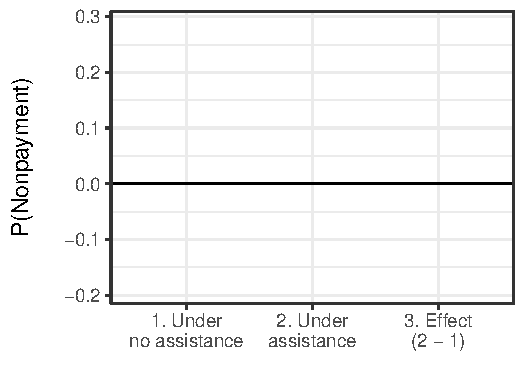
\includegraphics[height = .8\textheight]{figures/effect_public_nonpayment_0_}};
\node<2> at (0,0) {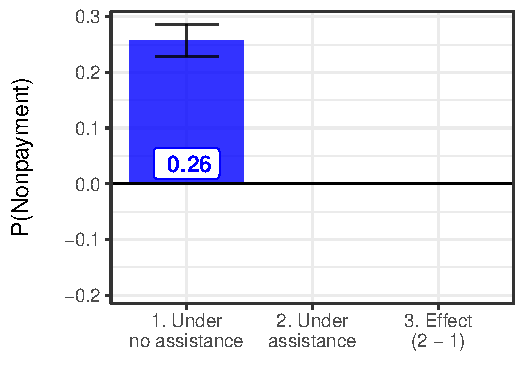
\includegraphics[height = .8\textheight]{figures/effect_public_nonpayment_1_}};
\node<3> at (0,0) {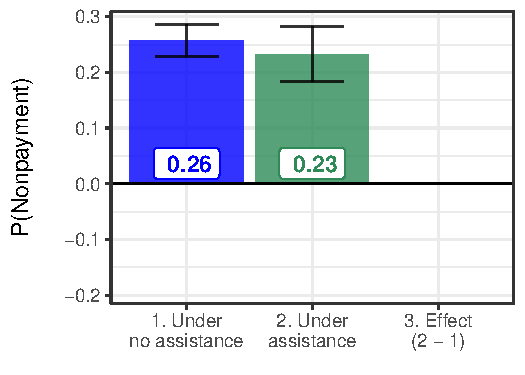
\includegraphics[height = .8\textheight]{figures/effect_public_nonpayment_2_}};
\node<4> at (0,0) {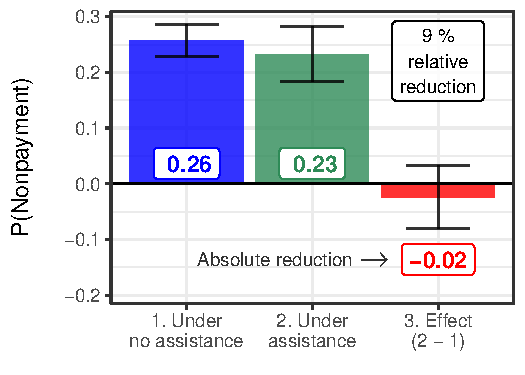
\includegraphics[height = .8\textheight]{figures/effect_public_nonpayment_3_}};
\end{tikzpicture}
\end{frame}

\begin{frame}{Effect of \bblue{other assistance} on \bblue{nonpayment}}
\centering
\begin{tikzpicture}
\node at (0,0) {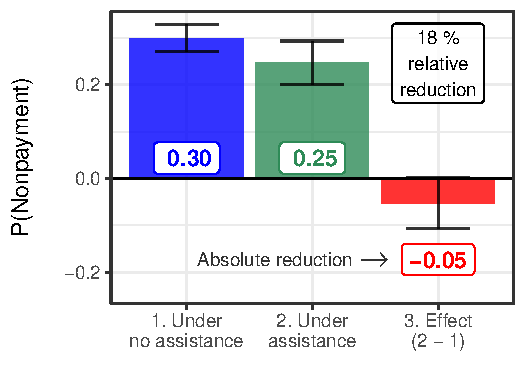
\includegraphics[height = .8\textheight]{figures/effect_assistance_nonpayment_3_}};
\end{tikzpicture}
\end{frame}

\begin{frame}{Effect of \bblue{public housing} on \bblue{eviction}}
\centering
\begin{tikzpicture}
\node at (0,0) {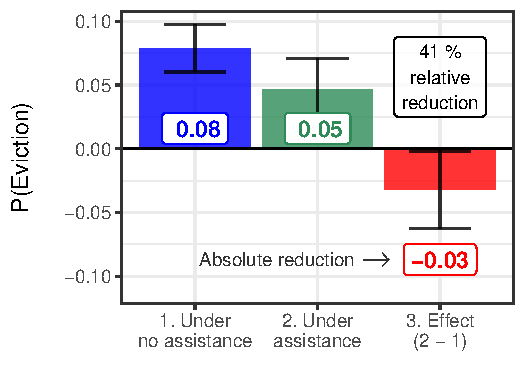
\includegraphics[height = .8\textheight]{figures/effect_public_evicted_3_}};
\end{tikzpicture}
\end{frame}

\begin{frame}{Effect of \bblue{other assistance} on \bblue{eviction}}
\centering
\begin{tikzpicture}
\node at (0,0) {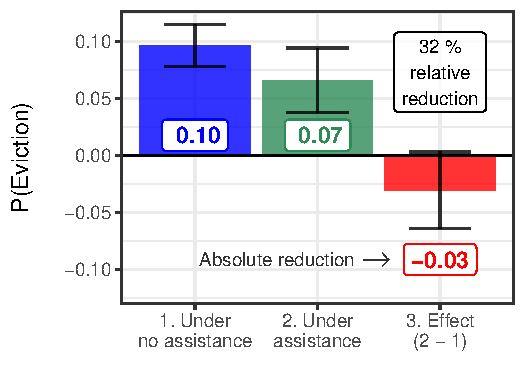
\includegraphics[height = .8\textheight]{figures/effect_assistance_evicted_3_}};
\end{tikzpicture}
\end{frame}

\begin{frame}
\centering
\begin{tikzpicture}
%\node<2> at (0,0) {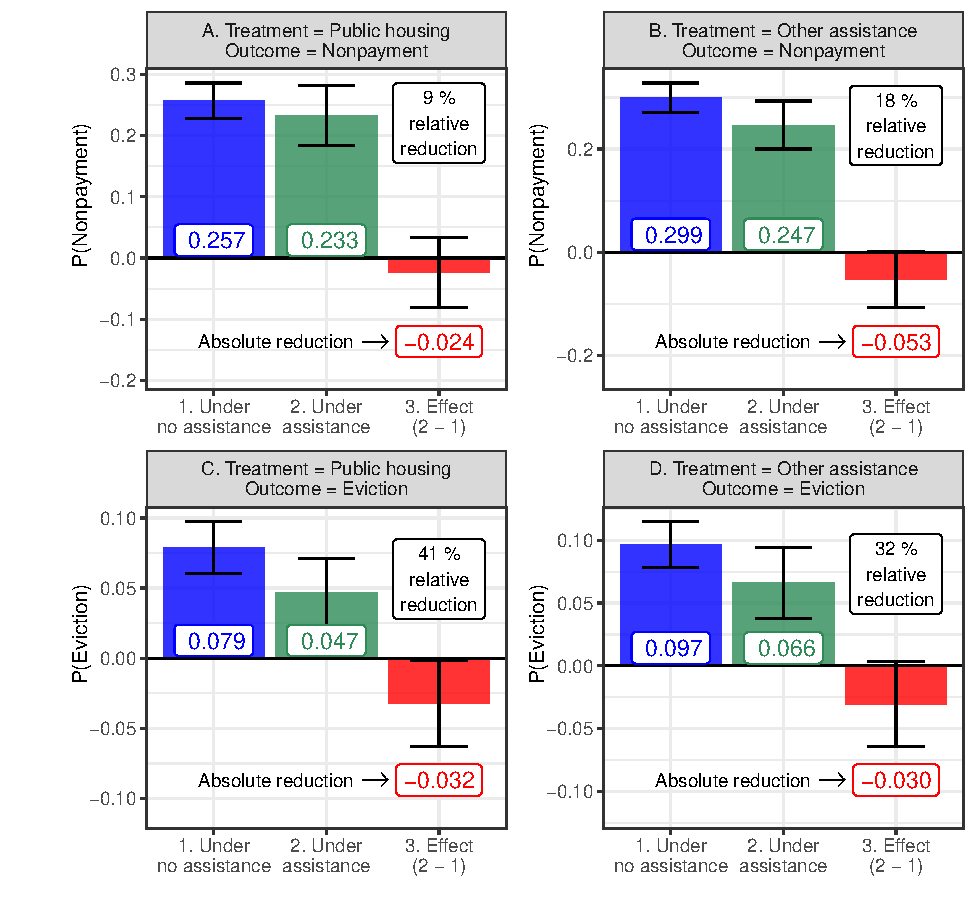
\includegraphics[height = .8\textheight, trim = .4in 3in 3in .05in, clip]{figures/effects_plot}};
%\node<3> at (0,0) {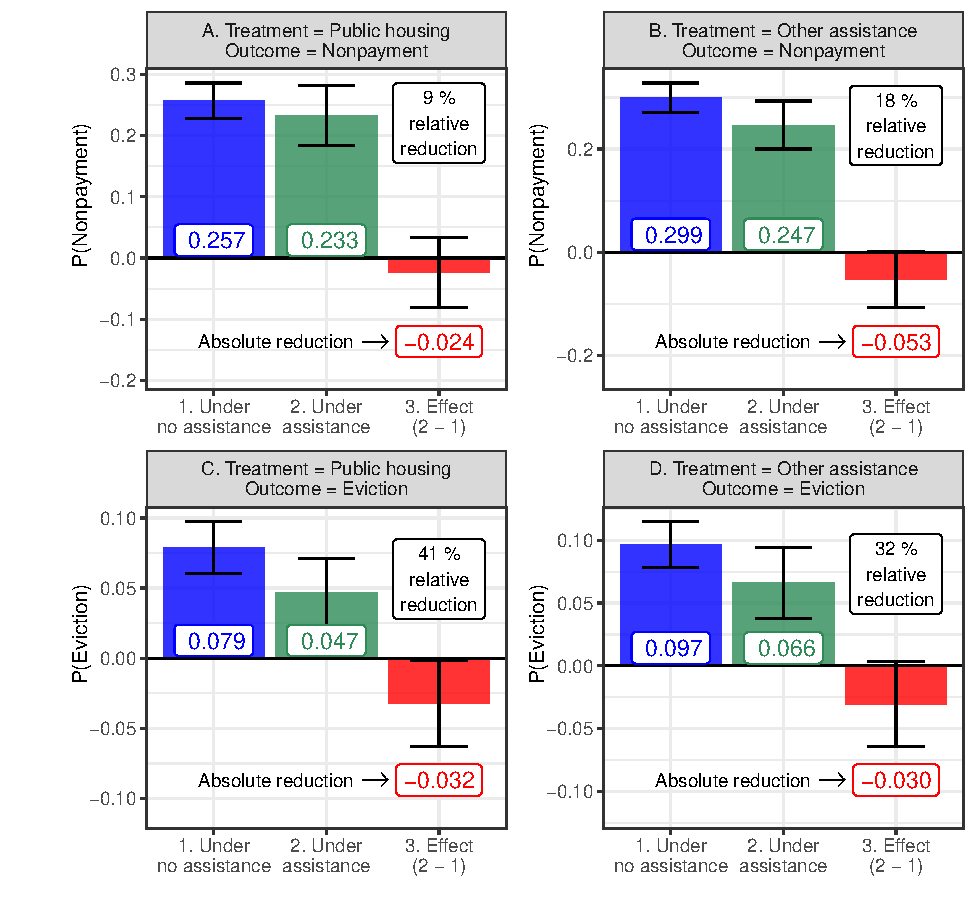
\includegraphics[height = .8\textheight, trim = 3.5in 3in 0 .05in, clip]{figures/effects_plot}};
%\node<4> at (0,0) {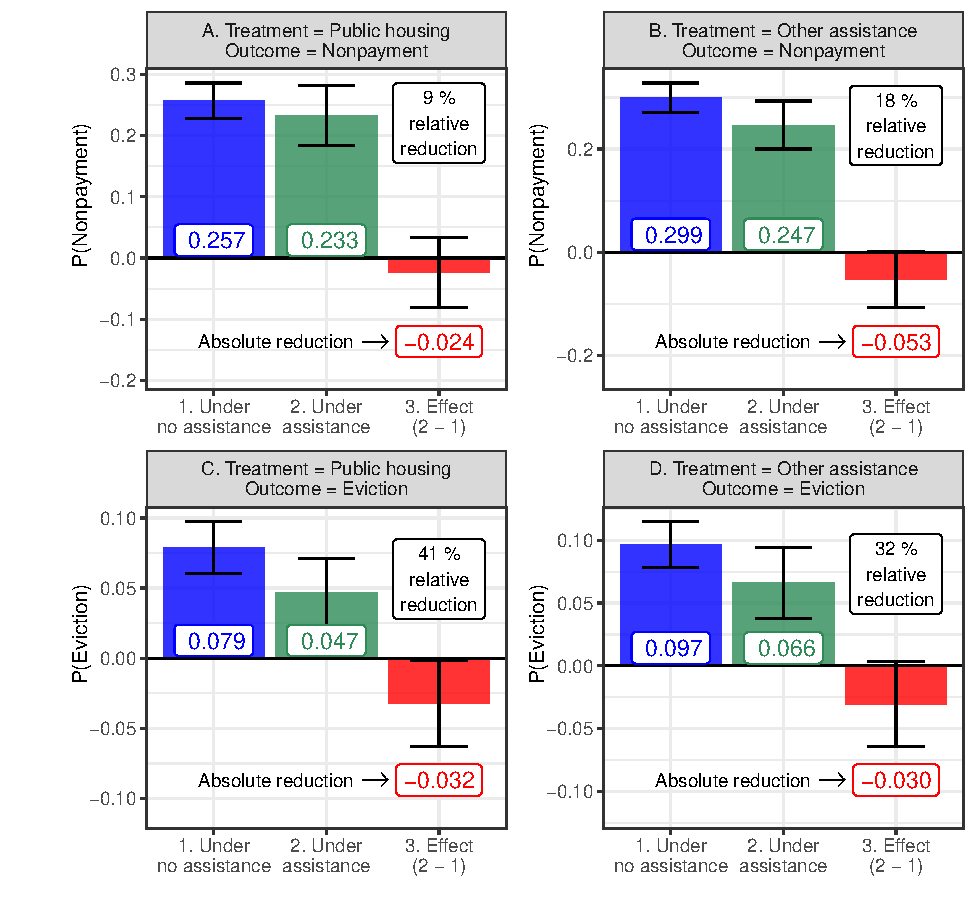
\includegraphics[height = .8\textheight, trim = .4in 0 3in 2.97in, clip]{figures/effects_plot}};
%\node<5> at (0,0) {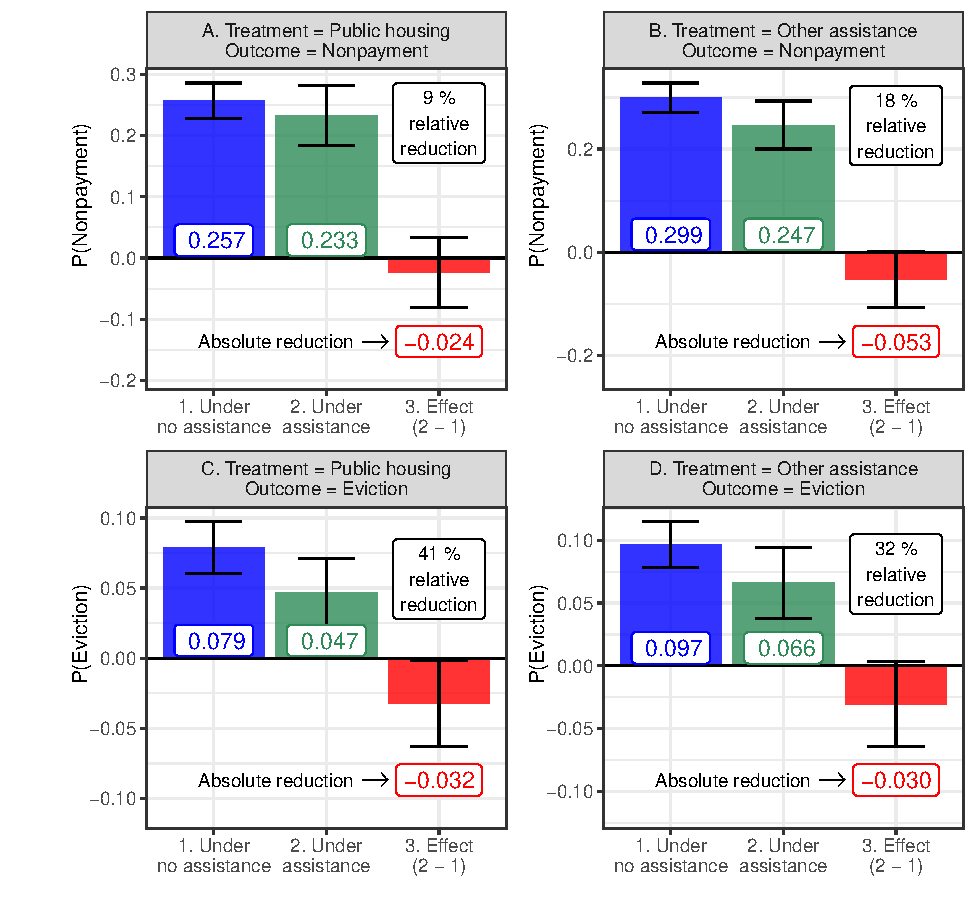
\includegraphics[height = .8\textheight, trim = 3.5in 0 0 2.97in, clip]{figures/effects_plot}};
\node at (0,0) {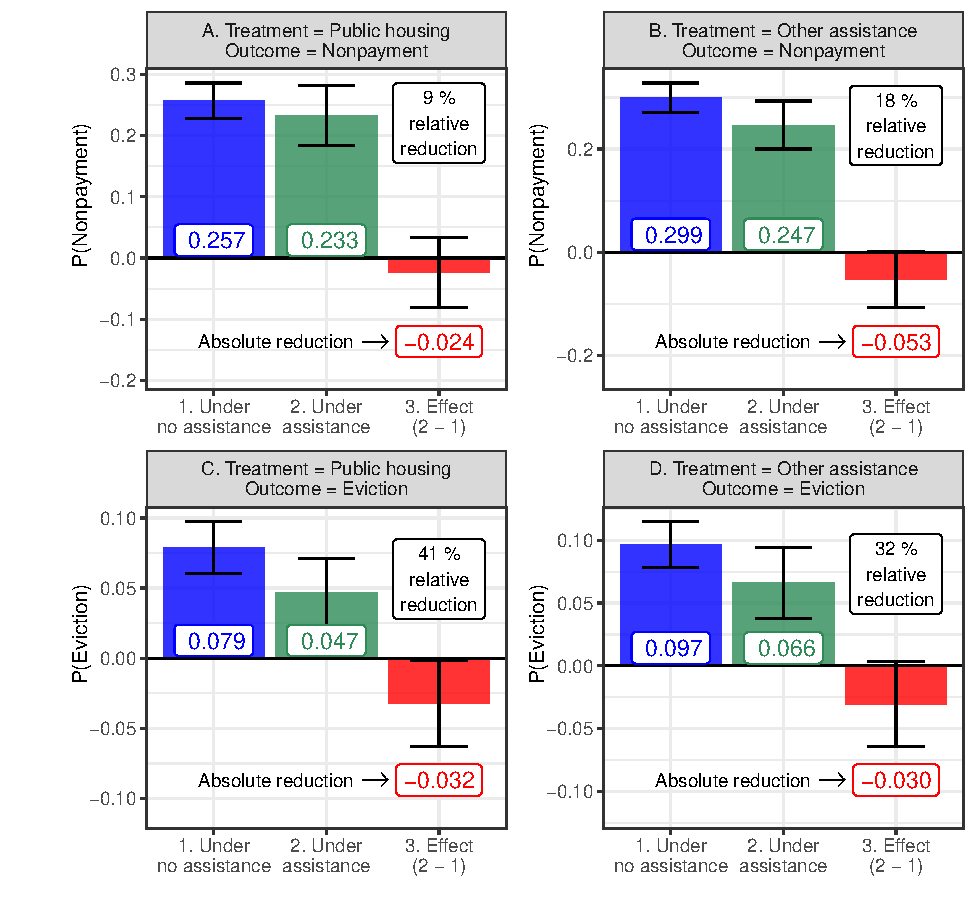
\includegraphics[height = \textheight]{figures/effects_plot}};
%\draw[rounded corners, thick] (-8,0.1) rectangle (9,9);
%\node at (.5,8.25) {$F$-test jointly testing red effect bars: $p = .020$};
%\draw[rounded corners, thick] (-8,0.1) rectangle (9,-9);
%\node at (.5,-8.25) {$F$-test jointly testing red effect bars: $p = .003$};
\end{tikzpicture}
\end{frame}
%\begin{frame}{What we found}
%\resizebox{!}{.7\textheight}{
%\begin{tikzpicture}
%\node at (0,0) {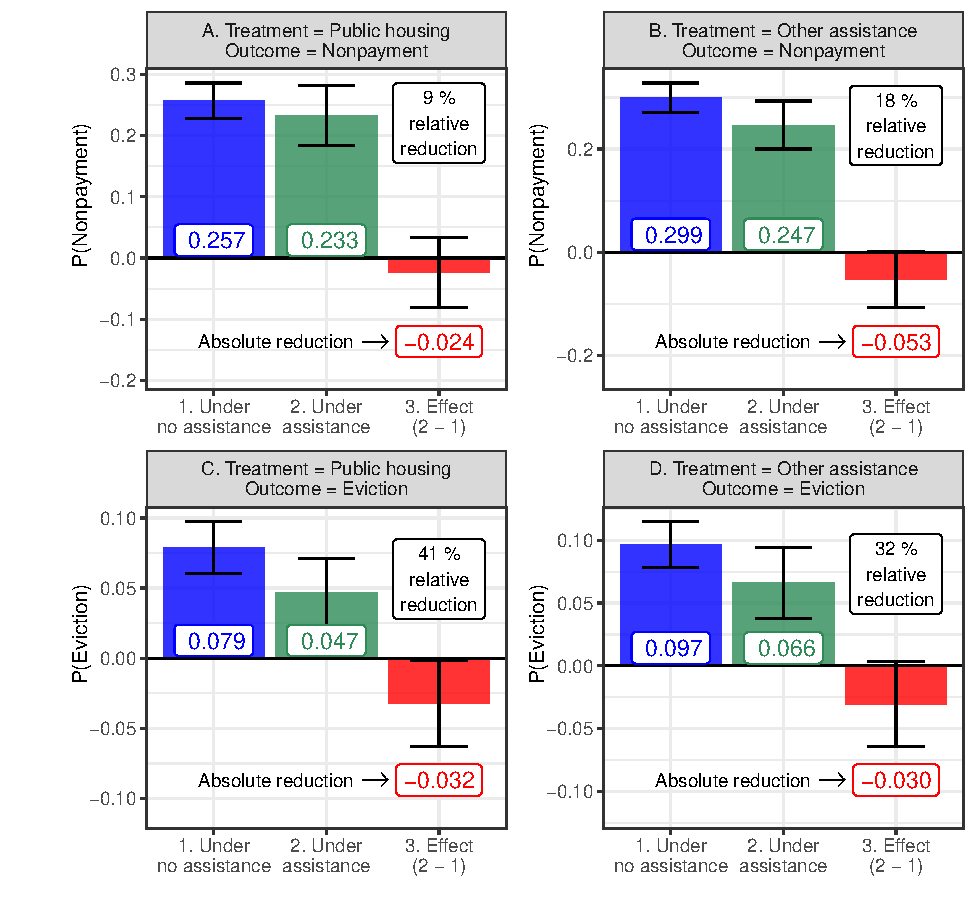
\includegraphics{figures/effects_plot}};
%\draw[rounded corners, thick] (-8,0.1) rectangle (9,9);
%\node at (.5,8.25) {$F$-test jointly testing red effect bars: $p = .020$};
%\draw[rounded corners, thick] (-8,0.1) rectangle (9,-9);
%\node at (.5,-8.25) {$F$-test jointly testing red effect bars: $p = .003$};
%\end{tikzpicture}
%}
%\end{frame}

\begin{frame}{Why this is important}
Families are struggling to pay rent and are being evicted. \pause \\
We should do something about it. \pause \\
We first need to know if existing policies are working. \vskip .5cm \pause
There are limitations
\begin{itemize}
\item Observational data
\item Small sample size
\end{itemize} \vskip .5cm \pause
But public housing cuts eviction prevalence \bblue{nearly in half}. \pause \\
\begin{itemize}
\item Warrants the cost of an experimental evaluation
\item Policy lever may be useful while evidence base grows
\end{itemize}
\end{frame}

\begin{frame}{References}
\tiny
\bibliography{FF_housing_assistance.bib}
\end{frame}

\end{document}